\chapter{अनुमापन विधियाँ और वक्र}\label{ch:b1:titration-methods}

एक औषधविक्रेता को \qty{500}{mg} लेबल वाली विटामिन C की गोलियों का एक खेप
मिलता है और उसे बेचने से पहले प्रमाणित करना है कि हर गोली में उतना ही है
जितना लेबल कहता है। वह विटामिन को सीधे नहीं तौलेगी: वह बंधकों और भराव-पदार्थों के साथ
मिला हुआ है। वह उसका \omterm{def:b1:titration-methods:titration}{अनुमापन} करेगी --- उसे ज्ञात सांद्रता वाले किसी अभिकर्मक से
अभिक्रिया कराएगी, आवश्यक आयतन मापेगी, और मात्रा परिकलित करेगी। कौन-सी अभिक्रिया,
उसका अंत कैसे दिखे, और परिणाम कितना निश्चित है: ये इस अध्याय के प्रश्न हैं, जो
पिछले पाँच अध्यायों के साम्यों को प्रयोगशाला की मेज़ पर ले आता है।

\begin{recall}
विद्यालय के खंड (कक्षा 11 और 12) ने रंग-परिवर्तन के साथ क्षारकों द्वारा अम्लों का
\omterm{def:b1:titration-methods:titration}{अनुमापन} किया था, pH मीटर और चालकता मीटर से \omterm{def:b1:titration-methods:titration}{अनुमापनों} का अनुसरण किया था,
और \omterm{def:b1:titration-methods:titration}{तुल्यता} संबंध $C_AV_A = C_BV_B$ का उपयोग किया था। प्रधान-अभिक्रिया
विधि \cref{ch:b1:predominant-reaction} में है;
अवक्षेपण, संकुलन और अपचयोपचय साम्य
\cref{ch:b1:precipitation,ch:b1:complexation,ch:b1:nernst} में।
\end{recall}

\begin{omfigure}
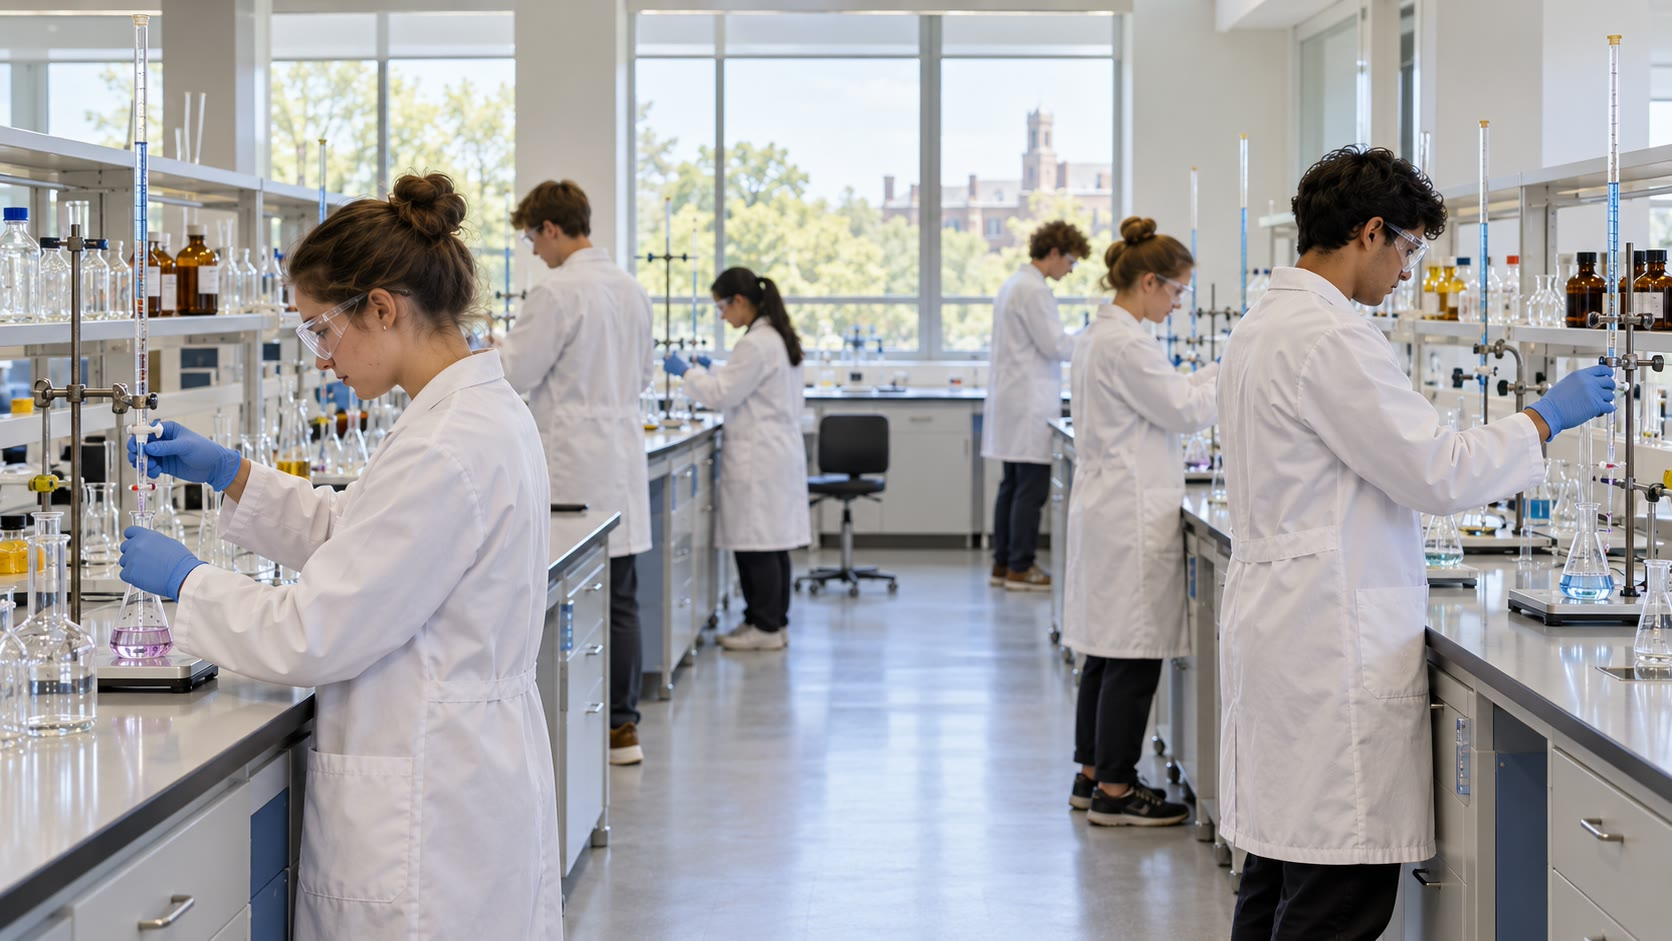
\includegraphics[width=0.66\linewidth]{images/book2/ai/b1-15-teaching-lab.jpg}

{\small एक शिक्षण प्रयोगशाला: ब्यूरेट, चुंबकीय विलोडक पर
शंक्वाकार फ़्लास्क, दस्ताने और चश्मे। \omterm{def:b1:titration-methods:titration}{अनुमापन} रसायन में सबसे सामान्य मात्रात्मक
मापन है।}
\end{omfigure}

\section{अनुमापन और तुल्यता}

\begin{definition}[अनुमापन, तुल्यता]\label{def:b1:titration-methods:titration}
\emph{अनुमापन}\index{अनुमापन} किसी स्पीशीज़ की मात्रा,
जिसे \emph{विश्लेष्य}\index{विश्लेष्य} कहते हैं, ज्ञात
सांद्रता वाले किसी अभिकर्मक, यानी \emph{अनुमापक}\index{अनुमापक}, से अभिक्रिया द्वारा
निर्धारित करता है, जिसे धीरे-धीरे मिलाया जाता है।
अभिक्रिया एकल, \omterm{def:b1:extent-q-and-k:quantitative}{मात्रात्मक} ($K$ बड़ा) और तीव्र होनी चाहिए।
\emph{तुल्यता}\index{तुल्यता} तब प्राप्त होती है जब अनुमापक और विश्लेष्य
अभिक्रिया के रससमीकरणमितीय अनुपात में एक साथ लाए जा चुके हों; तब मिलाया गया आयतन
तुल्यता आयतन है, और उस आयतन पर अनुमापन वक्र का बिंदु \emph{तुल्यता
बिंदु}\index{तुल्यता बिंदु} है। जिस आयतन पर प्रयोगकर्ता
रुकता है, कोई रंग-परिवर्तन या वक्र में कोई मोड़ देखकर, वह \emph{अंत्य
बिंदु}\index{अंत्य बिंदु} है; अच्छी विधि उसे
तुल्यता से मिला देती है।
\end{definition}

\begin{proposition}[तुल्यता संबंध]\label{prop:b1:titration-methods:equivalence}
\omterm{def:b1:titration-methods:titration}{अनुमापन} अभिक्रिया $a\,\mathrm{A} + b\,\mathrm{B} \to \cdots$ के लिए, जिसमें
\omterm{def:b1:titration-methods:titration}{विश्लेष्य} A ($n_A$ mol) है और \omterm{def:b1:titration-methods:titration}{अनुमापक} B, सांद्रता $C_B$ पर, \omterm{def:b1:titration-methods:titration}{तुल्यता}
आयतन यह संबंध संतुष्ट करता है:
\[
  \frac{n_A}{a} = \frac{C_B V_{\mathrm{eq}}}{b} .
\]
\end{proposition}

\begin{proof}
मान लीजिए $x$ वह प्रगति है जो $V$ \omterm{def:b1:titration-methods:titration}{अनुमापक} मिलाने के बाद होती है। \omterm{def:b1:titration-methods:titration}{तुल्यता} से पहले B
सीमांत है और, अभिक्रिया \omterm{def:b1:extent-q-and-k:quantitative}{मात्रात्मक} होने से, $x = C_BV/b$; उसके बाद
A सीमांत है और $x = n_A/a$। \omterm{def:b1:titration-methods:titration}{तुल्यता} वह आयतन है जहाँ दोनों
एक साथ समाप्त होते हैं, $n_A - ax = 0$ और $C_BV - bx = 0$: $x$ का निरसन करने पर
संबंध मिलता है।
\end{proof}

\section{प्रत्यक्ष और अप्रत्यक्ष अनुमापन}

\begin{definition}[अनुमापन के प्रकार]\label{def:b1:titration-methods:kinds}
\emph{प्रत्यक्ष अनुमापन}\index{प्रत्यक्ष अनुमापन} में \omterm{def:b1:titration-methods:titration}{अनुमापक} स्वयं
\omterm{def:b1:titration-methods:titration}{विश्लेष्य} से अभिक्रिया करता है। \emph{पश्च अनुमापन}\index{पश्च अनुमापन} में
किसी अभिकर्मक का ज्ञात आधिक्य \omterm{def:b1:titration-methods:titration}{विश्लेष्य} में मिलाया जाता है, और बचे हुए आधिक्य का
\omterm{def:b1:titration-methods:titration}{अनुमापन} किया जाता है। जब किसी विलयन में कई \omterm{def:b1:titration-methods:titration}{विश्लेष्य} हों जो
बारी-बारी से \omterm{def:b1:titration-methods:titration}{अनुमापक} से अभिक्रिया करें, तो उन्हें \emph{क्रमिक
अनुमापनों}\index{क्रमिक अनुमापन} द्वारा मापा जाता है, एक \omterm{def:b1:titration-methods:titration}{तुल्यता} के बाद दूसरी;
जब वे एक साथ अभिक्रिया करके एक ही \omterm{def:b1:titration-methods:titration}{तुल्यता} दें, तो \emph{युगपत्
अनुमापन}\index{युगपत् अनुमापन} द्वारा, जो
केवल उनका योग देता है।
\end{definition}

\begin{method}[पश्च अनुमापन]\label{met:b1:titration-methods:back-titration}
इसका उपयोग तब कीजिए जब प्रत्यक्ष अभिक्रिया धीमी हो, जब \omterm{def:b1:titration-methods:titration}{विश्लेष्य} अस्थायी या
वाष्पशील हो, या जब कोई सूचक प्रत्यक्ष अभिक्रिया के अनुकूल न हो।
\begin{enumerate}
  \item अभिकर्मक R की ज्ञात मात्रा $n_R$, आधिक्य में, मिलाइए और उसे
        \omterm{def:b1:titration-methods:titration}{विश्लेष्य} A से पूरी तरह अभिक्रिया करने दीजिए ($\alpha\,\mathrm{A} + \rho\,\mathrm{R}$)।
  \item आधिक्य R का \omterm{def:b1:titration-methods:titration}{अनुमापक} T से ($\rho'\,\mathrm{R} +
        \tau\,\mathrm{T}$) \omterm{def:b1:titration-methods:titration}{तुल्यता} आयतन $V_T$ तक \omterm{def:b1:titration-methods:titration}{अनुमापन} कीजिए।
  \item $n_{R,\text{आधिक्य}} = \frac{\rho'}{\tau}C_TV_T$ परिकलित कीजिए, फिर
        $n_A = \frac{\alpha}{\rho}(n_R - n_{R,\text{आधिक्य}})$।
\end{enumerate}
\end{method}

सप्ताहांत समस्या इसी प्रकार विटामिन C का \omterm{def:b1:titration-methods:titration}{अनुमापन} करती है: ऐस्कॉर्बिक अम्ल आयोडीन के
आधिक्य को अपचित करता है, और बची हुई आयोडीन का थायोसल्फ़ेट से \omterm{def:b1:titration-methods:titration}{अनुमापन} किया जाता है।

\section{pH-मितीय अनुमापन और सूचक}

\begin{omfigure}
\begin{tikzpicture}[font=\small]
  \pic at (0,0) {stirrer};
  \pic at (0,0.18) {beaker={0.55}{omDef!14}};
  \pic at (0.2,2.45) {burette={0.75}{white}};
  \pic at (-0.45,0.45) {probe};
  \pic (m) at (-2.6,3.2) {meter={pH}};
  \draw[thick] (-0.45,3.45) to[out=90, in=0] (m-b);
  \node[anchor=west] at (0.65,6.2) {ब्यूरेट: NaOH, \qty{0.100}{mol/L}};
  \node[anchor=west] at (1.0,1.0) {अम्ल, $V_0 = \qty{10.0}{mL}$, तनु किया हुआ};
  \draw[<-, omProp, thick] (1.2,-0.25) -- (1.8,-0.25) node[anchor=west, text=black] {चुंबकीय विलोडक};
  \draw[<-, omProp, thick] (-0.62,2.4) -- (-1.5,2.0) node[anchor=east, text=black] {संयुक्त इलेक्ट्रोड};
\end{tikzpicture}

{\small एक pH-मितीय \omterm{def:b1:titration-methods:titration}{अनुमापन}। संयुक्त काँच इलेक्ट्रोड ब्यूरेट से हर बार मिलाने के बाद
pH मापता है; विलोडक विलयन को मिलाता है।
इलेक्ट्रोड को पहले दो \omterm{def:b1:predominant-reaction:buffer}{बफ़र विलयनों} से अंशांकित किया जाता है।}
\end{omfigure}

\begin{omfigure}
\begin{tikzpicture}
\begin{axis}[name=s,
  width=0.5\linewidth, height=5.6cm, xmin=0, xmax=20, ymin=0, ymax=14,
  axis x line=bottom, axis y line=left, xlabel={$V$ (mL)}, ylabel={pH},
  xtick={0,5,10,15,20}, ytick={0,2,4,6,8,10,12,14},
  tick label style={font=\small}, label style={font=\small}]
\addplot[omDef, very thick] table[x=V, y=pH] {figdata/out/bachelor-1-titration-curves-strong.dat};
\addplot[omProp, thick] table[x=V, y=pH] {figdata/out/bachelor-1-titration-curves-weak.dat};
\node[font=\scriptsize, omDef, anchor=south west] at (axis cs:6,0.2) {\ce{HCl}};
\node[font=\scriptsize, omProp, anchor=west] at (axis cs:0.4,6.4) {\ce{CH3COOH}};
\draw[dotted] (axis cs:5,0) -- (axis cs:5,4.76) -- (axis cs:0,4.76);
\node[font=\scriptsize, anchor=north] at (axis cs:2.5,4.7) {$\mathrm{p}K_a$};
\end{axis}
\begin{axis}[at={(s.east)}, anchor=west, xshift=1.2cm,
  width=0.5\linewidth, height=5.6cm, xmin=0, xmax=20, ymin=0, ymax=14,
  axis x line=bottom, axis y line=left, xlabel={$V$ (mL)}, ylabel={pH},
  xtick={0,5,10,15,20}, ytick={0,2,4,6,8,10,12,14},
  tick label style={font=\small}, label style={font=\small}]
\addplot[omMeth, very thick] table[x=V, y=pH] {figdata/out/bachelor-1-titration-curves-mixture.dat};
\node[font=\scriptsize, anchor=west, align=left] at (axis cs:10.8,6.0) {\ce{HCl} + \ce{CH3COOH}\\ दो तुल्यता बिंदु};
\end{axis}
\end{tikzpicture}

{\small बाएँ: हाइड्रोक्लोरिक अम्ल और एथेनोइक अम्ल, हर एक का \qty{10.0}{mL},
दोनों \qty{0.100}{mol/L} पर, जिनका \qty{0.100}{mol/L} सोडियम हाइड्रॉक्साइड से
\omterm{def:b1:titration-methods:titration}{अनुमापन} किया गया है। \omterm{def:b1:predominant-reaction:strong-acid}{दुर्बल अम्ल} में एक बफ़र क्षेत्र है, अर्ध-तुल्यता पर pH $=
\mathrm{p}K_a$, और \omterm{def:b1:titration-methods:titration}{तुल्यता बिंदु} pH 8.73 पर।
दाएँ: एक मिश्रण, हर अम्ल का \qty{0.050}{mol/L}: \omterm{def:b1:predominant-reaction:strong-acid}{प्रबल अम्ल} का
\omterm{def:b1:titration-methods:titration}{अनुमापन} पहले होता है (\omterm{def:b1:titration-methods:titration}{तुल्यता} \qty{5}{mL} पर), फिर \omterm{def:b1:predominant-reaction:strong-acid}{दुर्बल अम्ल} का
(\qty{10}{mL})।}
\end{omfigure}

\begin{proposition}[दुर्बल अम्ल की अर्ध-तुल्यता]\label{prop:b1:titration-methods:half-equivalence}
जब किसी \omterm{def:b1:predominant-reaction:strong-acid}{दुर्बल अम्ल} HA का किसी \omterm{def:b1:predominant-reaction:strong-acid}{प्रबल क्षारक} से \omterm{def:b1:titration-methods:titration}{अनुमापन} किया जाता है, तो अर्ध-तुल्यता पर
$\mathrm{pH} = \mathrm{p}K_a$, बशर्ते अम्ल न बहुत प्रबल हो
न बहुत तनु (\qty{0.1}{mol/L} पर $\mathrm{p}K_a$ लगभग 4 और 10 के बीच)।
\end{proposition}

\begin{proof}
अर्ध-तुल्यता पर \omterm{def:b1:extent-q-and-k:quantitative}{मात्रात्मक अभिक्रिया} \ce{HA + OH- -> A- + H2O}
HA के आधे भाग को बदल चुकी होती है: $[\mathrm{HA}] = [\mathrm{A^-}]$, और
हेंडरसन संबंध $\mathrm{pH} = \mathrm{p}K_a$ देता है। शर्त
यह सुनिश्चित करती है कि HA की पानी से अभिक्रिया और $\mathrm{A^-}$ की
पानी से अभिक्रिया उन मात्राओं को उल्लेखनीय रूप से नहीं बदलतीं।
\end{proof}

\begin{proposition}[दुर्बल अम्ल की तुल्यता पर pH]\label{prop:b1:titration-methods:ph-at-equivalence}
किसी \omterm{def:b1:predominant-reaction:strong-acid}{दुर्बल अम्ल} ($\mathrm{p}K_a$) की \omterm{def:b1:predominant-reaction:strong-acid}{प्रबल क्षारक} से \omterm{def:b1:titration-methods:titration}{तुल्यता} पर
विलयन संयुग्मी क्षारक है, सांद्रता $C'$ पर (तनुकरण के बाद), और
\[
  \mathrm{pH} = \tfrac12(\mathrm{p}K_e + \mathrm{p}K_a + \log C') .
\]
\end{proposition}

\begin{proof}
क्षारक की पानी से \omterm{def:b1:predominant-reaction:predominant-reaction}{प्रधान अभिक्रिया},
\ce{A- + H2O <=> HA + OH-}, का $K = K_e/K_a$ है; थोड़े क्षारक के
रूपांतरित होने पर $[\ce{OH-}] = \sqrt{KC'}$ (\cref{prop:b1:predominant-reaction:ph-formulas}),
जिससे परिणाम मिलता है। एथेनोइक अम्ल के लिए, $C' = \qty{0.050}{mol/L}$:
$\frac12(14.00 + 4.76 - 1.30) = 8.73$।
\end{proof}

\begin{proposition}[क्रमिक अनुमापन]\label{prop:b1:titration-methods:successive}
एक ही क्षारक से अनुमापित दो अम्ल अलग-अलग \omterm{def:b1:titration-methods:titration}{तुल्यताएँ} देते हैं, हर एक
\qty{1}{\percent} से बेहतर, यदि उनके $\mathrm{p}K_a$ में कम-से-कम 4 का अंतर हो।
\end{proposition}

\begin{proof}
पहली \omterm{def:b1:titration-methods:titration}{तुल्यता} पर क्षारक $\mathrm{A_1^-}$ की
दूसरे अम्ल $\mathrm{HA_2}$ से अभिक्रिया, $\mathrm{A_1^-} + \mathrm{HA_2}
\rightleftharpoons \mathrm{HA_1} + \mathrm{A_2^-}$, का $K = 10^{\mathrm{p}K_1 - \mathrm{p}K_2}$ है।
बराबर मात्राओं से आरंभ करने पर दूसरे अम्ल का पहले से अनुमापित भिन्न $x$
$x^2/(1 - x)^2 = K$ को संतुष्ट करता है; $x \leqslant 0.01$ के लिए $K
\leqslant 10^{-4}$, अर्थात् $\mathrm{p}K_2 - \mathrm{p}K_1 \geqslant 4$।
\end{proof}

फ़ॉस्फ़ोरिक अम्ल (2.15, 7.21, 12.34) दो स्पष्ट \omterm{def:b1:titration-methods:titration}{तुल्यताएँ} देता है; तीसरी
क्षारक के पानी में खो जाती है। हाइड्रोक्लोरिक अम्ल के साथ मिला एथेनोइक अम्ल
(चित्र में दाएँ) उसके बाद अनुमापित होता है, क्योंकि \omterm{def:b1:predominant-reaction:strong-acid}{प्रबल
अम्ल} व्यवहार में 0 से नीचे $\mathrm{p}K_a$ वाला होता है।

\begin{method}[वक्र पर तुल्यता खोजना]\label{met:b1:titration-methods:derivative}
\begin{enumerate}
  \item अवकलज: क्रमिक बिंदुओं के बीच $\Delta\mathrm{pH}/\Delta V$ परिकलित
        कीजिए; \omterm{def:b1:titration-methods:titration}{तुल्यता} उसके उच्चिष्ठ पर है।
  \item स्पर्शरेखाएँ: उछाल के दोनों ओर वक्र पर दो समांतर स्पर्शरेखाएँ
        खींचिए, और उनसे समदूरस्थ समांतर रेखा; यह
        वक्र को \omterm{def:b1:titration-methods:titration}{तुल्यता बिंदु} पर काटती है।
\end{enumerate}
\end{method}

\begin{method}[स्पर्शरेखाएँ, परिकलन द्वारा]\label{met:b1:titration-methods:tangents}
कंप्यूटर द्वारा दर्ज वक्र के लिए उछाल के हर ओर के बिंदुओं पर
एक चिकना फलन फ़िट कीजिए और नति-परिवर्तन बिंदु लीजिए; सममित
उछाल (\omterm{def:b1:predominant-reaction:strong-acid}{प्रबल अम्ल}, \omterm{def:b1:predominant-reaction:strong-acid}{प्रबल क्षारक}) के लिए pH 7 पर उछाल का
मध्य-बिंदु ही \omterm{def:b1:titration-methods:titration}{तुल्यता बिंदु} है।
\end{method}

\begin{definition}[रंग सूचक, रंग-परिवर्तन परास]\label{def:b1:titration-methods:indicator}
\emph{रंग सूचक}\index{रंग सूचक} एक दुर्बल \omterm{def:b1:predominant-reaction:bronsted}{अम्ल--क्षारक
युग्म} HIn/In$^-$ है जिसके दोनों रूपों के रंग भिन्न हों। इसका रंग
\emph{रंग-परिवर्तन परास}\index{रंग-परिवर्तन परास} में बदलता है, वह pH परास जहाँ
कोई भी रूप स्पष्ट रूप से प्रभावी नहीं होता, लगभग $\mathrm{p}K_{a}(\mathrm{HIn}) \pm 1$।
\end{definition}

\begin{omfigure}
\begin{tabular}{lccl}
\hline
सूचक & $\mathrm{p}K_a$ & \omterm{def:b1:titration-methods:indicator}{रंग-परिवर्तन परास} & रंग (अम्ल / क्षारक) \\
\hline
मेथिल ऑरेंज & 3.5 & 2.5--4.5 & लाल / पीला \\
मेथिल रेड & 4.8 & 3.8--5.8 & लाल / पीला \\
फ़ीनॉल रेड & 7.9 & 6.9--8.9 & पीला / लाल \\
थाइमॉल ब्लू (दूसरा परिवर्तन) & 9.2 & 8.2--10.2 & पीला / नीला \\
\hline
\end{tabular}

\smallskip
{\small चार सूचक, जिनके $\mathrm{p}K_a$ \omterm{def:b1:complexation:formation-constant}{वियोजन स्थिरांकों} के एक समालोचनात्मक संकलन से
लिए गए हैं; \omterm{def:b1:titration-methods:indicator}{रंग-परिवर्तन परास} $\mathrm{p}K_a \pm 1$ हैं।}
% ledger: pka:methylorange, pka:methylred, pka:phenolred, pka:thymolblue2
\end{omfigure}

\begin{method}[सूचक चुनना]\label{met:b1:titration-methods:choose-indicator}
ऐसा सूचक चुनिए जिसका \omterm{def:b1:titration-methods:indicator}{रंग-परिवर्तन परास} वक्र के ऊर्ध्वाधर उछाल के भीतर हो,
\omterm{def:b1:titration-methods:titration}{तुल्यता} के pH के यथासंभव निकट। \omterm{def:b1:predominant-reaction:strong-acid}{प्रबल अम्ल} का
\omterm{def:b1:predominant-reaction:strong-acid}{प्रबल क्षारक} से \omterm{def:b1:titration-methods:titration}{अनुमापन} (यहाँ $\pm\qty{0.1}{mL}$ के लिए उछाल 3.3 से 10.7): चारों में से
कोई भी। एथेनोइक अम्ल (\omterm{def:b1:titration-methods:titration}{तुल्यता} 8.73): फ़ीनॉल रेड या थाइमॉल ब्लू; मेथिल
ऑरेंज \omterm{def:b1:titration-methods:titration}{तुल्यता} से बहुत पहले रंग बदल देगा।
\end{method}

\section{विभवमितीय अनुमापन}

\begin{definition}[विभवमितीय अनुमापन]\label{def:b1:titration-methods:potentiometric}
\emph{विभवमितीय अनुमापन}\index{विभवमितीय अनुमापन}
विलयन में किसी इलेक्ट्रोड के विभव का, किसी \omterm{def:b1:nernst:reference-electrode}{संदर्भ इलेक्ट्रोड} के सापेक्ष,
अनुसरण करता है, अपचयोपचय (प्लैटिनम का तार), अवक्षेपण (सिल्वर का
तार) या संकुलन \omterm{def:b1:titration-methods:titration}{अनुमापन} के लिए।
\end{definition}

\begin{proposition}[अपचयोपचय अनुमापन के विशिष्ट बिंदु]\label{prop:b1:titration-methods:potentiometric-points}
$\mathrm{Red_1}$ के $\mathrm{Ox_2}$ द्वारा \omterm{def:b1:titration-methods:titration}{अनुमापन} के लिए, अभिक्रिया
$n_2\,\mathrm{Red_1} + n_1\,\mathrm{Ox_2} \to n_2\,\mathrm{Ox_1} +
n_1\,\mathrm{Red_2}$ के साथ (क्रमशः $n_1$ और $n_2$ इलेक्ट्रॉनों के युग्म), $E(V_{\mathrm{eq}}/2) = E^\circ_1$, $E(2V_{\mathrm{eq}}) =
E^\circ_2$, और \omterm{def:b1:titration-methods:titration}{तुल्यता} पर
\[
  E_{\mathrm{eq}} = \frac{n_1E^\circ_1 + n_2E^\circ_2}{n_1 + n_2},
\]
उन युग्मों के लिए जिनके \omterm{def:b1:nernst:couple}{अर्ध-समीकरणों} में कोई अन्य स्पीशीज़ न हो (या ऐसे pH पर
जो अतिरिक्त पदों को स्थिर रखे)।
\end{proposition}

\begin{proof}
अर्ध-तुल्यता पर $\mathrm{Red_1}$ का आधा भाग ऑक्सीकृत हो चुका है:
$[\mathrm{Ox_1}] = [\mathrm{Red_1}]$ और युग्म 1 का \omterm{thm:b1:nernst:nernst}{नेर्न्स्ट समीकरण}
$E^\circ_1$ देता है। $2V_{\mathrm{eq}}$ पर $\mathrm{Ox_2}$ उतनी ही मात्रा में आधिक्य में है
जितनी अपचित हुई थी: $[\mathrm{Ox_2}] = [\mathrm{Red_2}]$, $E = E^\circ_2$।
\omterm{def:b1:titration-methods:titration}{तुल्यता} पर युग्म 1 के \omterm{thm:b1:nernst:nernst}{नेर्न्स्ट समीकरण} को $n_1$ से और
युग्म 2 के समीकरण को $n_2$ से गुणा करके जोड़िए; रससमीकरणमिति से
$[\mathrm{Ox_1}]/[\mathrm{Red_1}] \cdot [\mathrm{Ox_2}]/[\mathrm{Red_2}] = 1$ होता है
(बचे हुए $\mathrm{Red_1}$ और $\mathrm{Ox_2}$ की मात्राएँ उसी
अनुपात में हैं जिसमें उत्पाद), इसलिए लघुगणक कट जाते हैं।
\end{proof}

\qty{1}{mol/L} अम्ल में परमैंगनेट द्वारा आयरन(II) के लिए $n_1 = 1$ और $n_2 =
5$: $E_{\mathrm{eq}} = (0.77 + 5 \times 1.51)/6 = 1.39$~V। उछाल, लगभग
0.8 से 1.5~V तक, इतना बड़ा है कि \omterm{def:b1:titration-methods:titration}{अंत्य बिंदु} तीक्ष्ण होता है; व्यवहार में
परमैंगनेट स्वयं अपना सूचक है, उसका बैंगनी रंग आधिक्य की पहली बूँद पर
बना रहता है।

\begin{omfigure}
\begin{tikzpicture}
\begin{axis}[name=p,
  width=0.5\linewidth, height=5.6cm, xmin=0, xmax=20, ymin=0.6, ymax=1.6,
  axis x line=bottom, axis y line=left, xlabel={$V$ (mL)}, ylabel={$E$ (V)},
  xtick={0,5,10,15,20},
  tick label style={font=\small}, label style={font=\small}]
\addplot[omDef, very thick] table[x=V, y=E] {figdata/out/bachelor-1-titration-curves-potentiometric.dat};
\draw[dotted] (axis cs:5,0.6) -- (axis cs:5,0.77) -- (axis cs:0,0.77);
\draw[dotted] (axis cs:10,0.6) -- (axis cs:10,1.39) -- (axis cs:0,1.39);
\node[font=\scriptsize, anchor=south west] at (axis cs:0.2,0.77) {0.77};
\node[font=\scriptsize, anchor=south west] at (axis cs:0.2,1.39) {1.39};
\end{axis}
\begin{axis}[at={(p.east)}, anchor=west, xshift=1.2cm,
  width=0.5\linewidth, height=5.6cm, xmin=0, xmax=20, ymin=0, ymax=4.6,
  axis x line=bottom, axis y line=left, xlabel={$V$ (mL)},
  ylabel={$\kappa$ (mS/cm)}, xtick={0,5,10,15,20},
  tick label style={font=\small}, label style={font=\small}]
\addplot[omProp, very thick] table[x=V, y=kappa] {figdata/out/bachelor-1-titration-curves-conductimetric.dat};
\draw[dotted] (axis cs:10,0) -- (axis cs:10,1.15);
\end{axis}
\end{tikzpicture}

{\small बाएँ: \qty{1}{mol/L} अम्ल में \qty{0.100}{mol/L} आयरन(II) के
\qty{10.0}{mL} का \qty{0.0200}{mol/L} परमैंगनेट द्वारा \omterm{def:b1:titration-methods:potentiometric}{विभवमितीय अनुमापन}
(प्लैटिनम इलेक्ट्रोड, हाइड्रोजन
इलेक्ट्रोड के सापेक्ष विभव)। दाएँ: \qty{0.0100}{mol/L}
हाइड्रोक्लोरिक अम्ल के \qty{100}{mL} का \qty{0.100}{mol/L} सोडियम हाइड्रॉक्साइड
द्वारा चालकतामितीय \omterm{def:b1:titration-methods:titration}{अनुमापन}; \omterm{def:b1:titration-methods:titration}{तुल्यता} दो सरल रेखाओं के
प्रतिच्छेदन पर है।}
% ledger: lam:H+, lam:OH-, lamsalt:HCl, lamsalt:NaCl (conductivities in figdata/bachelor-1/titration-curves.py)
\end{omfigure}

\section{चालकतामितीय, संकुलमितीय और अवक्षेपण अनुमापन}

\begin{definition}[मोलर आयनिक चालकता]\label{def:b1:titration-methods:conductivity}
किसी विलयन की चालकता $\kappa$ (\unit{S/m} में) यह मापती है कि वह अपने आयनों की
गति द्वारा कितनी अच्छी तरह धारा वहन करता है। किसी आयन की \emph{मोलर आयनिक
चालकता}\index{मोलर आयनिक चालकता} $\lambda_i$ प्रति इकाई आयतन प्रति मोल उसका
योगदान है; अनंत तनुता पर इसका मान,
$\lambda_i^\circ$, किसी दिए गए ताप पर आयन और विलायक का एक स्थिरांक है।
\end{definition}

\begin{proposition}[कोलराउश नियम]\label{prop:b1:titration-methods:kohlrausch}
तनु विलयन में चालकता आयनों के योगदानों का
योग है,
\[
  \kappa = \sum_i \lambda_i^\circ c_i ,
\]
जो \emph{कोलराउश नियम}\index{कोलराउश नियम} है; किसी लवण की मोलर चालकता
उसके आयनों की मोलर चालकताओं का योग है।
\end{proposition}

\admitted{\omterm{prop:b1:titration-methods:kohlrausch}{कोलराउश नियम} व्यक्त करता है कि तनु आयन स्वतंत्र रूप से
गति करते हैं; अधिक सांद्रता पर इसकी सीमाओं का अध्ययन द्वितीय वर्ष के
खंड में होता है। यहाँ हम इसे एक प्रायोगिक नियम के रूप में प्रयुक्त करते हैं।}

\begin{proposition}[चालकतामितीय अनुमापन की प्रवणताएँ]\label{prop:b1:titration-methods:conductimetric-slopes}
जब किसी \omterm{def:b1:predominant-reaction:strong-acid}{प्रबल अम्ल} H$^+$X$^-$ का किसी \omterm{def:b1:predominant-reaction:strong-acid}{प्रबल क्षारक}
Na$^+$OH$^-$ से बड़े आयतन में \omterm{def:b1:titration-methods:titration}{अनुमापन} किया जाता है (तनुकरण नगण्य), तो चालकता
मिलाए गए आयतन के साथ रैखिक रूप से बदलती है, और प्रवणता \omterm{def:b1:titration-methods:titration}{तुल्यता} से पहले
$\lambda^\circ(\ce{Na+}) - \lambda^\circ(\ce{H+}) < 0$ के समानुपाती होती है
और बाद में $\lambda^\circ(\ce{Na+}) + \lambda^\circ(\ce{OH-}) > 0$ के।
\end{proposition}

\begin{proof}
\omterm{def:b1:titration-methods:titration}{तुल्यता} से पहले मिलाए गए हाइड्रॉक्साइड का हर मोल \ce{H+} का एक मोल हटाता है
(\ce{H+ + OH- -> H2O}) और \ce{Na+} का एक मोल लाता है; \omterm{def:b1:titration-methods:titration}{तुल्यता} के
बाद वह एक \ce{Na+} और एक \ce{OH-} जोड़ता है। \ce{X-} अपरिवर्तित रहता है।
\omterm{prop:b1:titration-methods:kohlrausch}{कोलराउश नियम} के अनुसार चालकता $\lambda^\circ$ के उन संयोजनों गुणा
मिलाई गई मात्रा भाग (स्थिर) आयतन से बदलती है।
\end{proof}

सीमांत चालकताओं, $\lambda^\circ(\ce{H+}) =
\qty{349.8}{S.cm^2/mol}$ और $\lambda^\circ(\ce{OH-}) = 198.3$, और
लवणों \ce{HCl} (426) और \ce{NaCl} (126.5) की चालकताओं से \omterm{prop:b1:titration-methods:kohlrausch}{कोलराउश नियम}
$\lambda^\circ(\ce{Cl-}) = 426 - 349.8 = 76.2$ और $\lambda^\circ(\ce{Na+}) =
126.5 - 76.2 = 50.3$~\unit{S.cm^2/mol} देता है। हाइड्रोजन और हाइड्रॉक्साइड आयन
दूसरों से कहीं बेहतर चालन करते हैं: वक्र एक तीक्ष्ण V है।

संकुलमितीय \omterm{def:b1:titration-methods:titration}{अनुमापन} ईडीटीए का उपयोग करते हैं: pH 10 (अमोनिया बफ़र) पर कैल्सियम
और मैग्नीशियम उससे \omterm{def:b1:extent-q-and-k:quantitative}{मात्रात्मक} रूप से अभिक्रिया करते हैं (\cref{ch:b1:complexation} के
सशर्त स्थिरांक), और एक सूचक जो स्वयं धातु का दुर्बल
संकुलक है, तब रंग बदलता है जब ईडीटीए उससे अंतिम
धातु आयन छीन लेता है --- पानी की कठोरता का \omterm{def:b1:titration-methods:titration}{अनुमापन}। अवक्षेपण
\omterm{def:b1:titration-methods:titration}{अनुमापन} सिल्वर आयनों का उपयोग करते हैं: क्लोराइड का सिल्वर नाइट्रेट से \omterm{def:b1:titration-methods:titration}{अनुमापन}
क्रोमेट को सूचक बनाकर किया जाता है (\cref{exo:b1:precipitation:8}), या
सिल्वर इलेक्ट्रोड से उसका अनुसरण किया जाता है (\cref{ch:b1:nernst})। इन सभी परिणामों की
परिशुद्धता, जो काँच के उपकरणों और \omterm{def:b1:titration-methods:titration}{अंत्य बिंदु} से तय होती है,
\cref{ch:b1:lab-techniques-1} में दी गई है।

\section{अभ्यास}

\begin{exercise}[$\star$]\label{exo:b1:titration-methods:1}
सोडियम हाइड्रॉक्साइड विलयन के \qty{20.0}{mL} के लिए \qty{0.100}{mol/L}
हाइड्रोक्लोरिक अम्ल के \qty{12.4}{mL} लगते हैं। अभिक्रिया, उसका स्थिरांक लिखिए,
और क्षारक की सांद्रता परिकलित कीजिए।
\end{exercise}

\begin{exercise}[$\star$]\label{exo:b1:titration-methods:2}
\qty{0.10}{mol/L} हाइड्रोक्लोरिक अम्ल द्वारा अमोनिया (\qty{0.10}{mol/L},
$\mathrm{p}K_a = 9.25$) के \omterm{def:b1:titration-methods:titration}{अनुमापन} के लिए सारणी का कौन-सा सूचक उपयुक्त है? पहले
\omterm{def:b1:titration-methods:titration}{तुल्यता} पर pH परिकलित कीजिए।
\end{exercise}

\begin{exercise}[$\star$]\label{exo:b1:titration-methods:3}
आयरन(II) के \qty{10.0}{mL} का \qty{0.0200}{mol/L} परमैंगनेट से
\omterm{def:b1:titration-methods:titration}{अनुमापन} किया जाता है; बैंगनी रंग \qty{12.6}{mL} से बना रहता है।
अभिक्रिया लिखिए और आयरन(II) की सांद्रता परिकलित कीजिए।
\end{exercise}

\begin{exercise}[$\star$]\label{exo:b1:titration-methods:4}
पानी के \qty{50.0}{mL} नमूने का pH 10 पर \qty{0.0100}{mol/L} ईडीटीए से
\omterm{def:b1:titration-methods:titration}{अनुमापन} किया जाता है; \omterm{def:b1:titration-methods:titration}{तुल्यता} \qty{14.2}{mL} पर है। ईडीटीए
कैल्सियम और मैग्नीशियम से एक-एक के अनुपात में अभिक्रिया करता है। इन दोनों आयनों की कुल
सांद्रता परिकलित कीजिए। यह \omterm{def:b1:titration-methods:kinds}{युगपत् अनुमापन} है या क्रमिक?
\end{exercise}

\begin{exercise}[$\star\star$]\label{exo:b1:titration-methods:5}
\qty{0.100}{mol/L} सोडियम हाइड्रॉक्साइड द्वारा \qty{0.100}{mol/L}
एथेनोइक अम्ल के \qty{10.0}{mL} के \omterm{def:b1:titration-methods:titration}{अनुमापन} के लिए, 0, 5.0, 10.0
और \qty{15.0}{mL} पर pH, \cref{ch:b1:predominant-reaction} की विधियों से परिकलित कीजिए,
और इस अध्याय के वक्र से तुलना कीजिए।
\end{exercise}

\begin{exercise}[$\star\star$]\label{exo:b1:titration-methods:6}
दिखाइए कि सोडियम हाइड्रॉक्साइड द्वारा फ़ॉस्फ़ोरिक अम्ल का pH-मितीय \omterm{def:b1:titration-methods:titration}{अनुमापन}
दो उछाल देता है, और \qty{0.100}{mol/L} अम्ल (\qty{10.0}{mL}, क्षारक \qty{0.100}{mol/L})
के लिए हर \omterm{def:b1:titration-methods:titration}{तुल्यता} पर pH परिकलित कीजिए। तीसरा उछाल
क्यों नहीं है?
\end{exercise}

\begin{exercise}[$\star\star$]\label{exo:b1:titration-methods:7}
हाइड्रोक्लोरिक अम्ल और एथेनोइक अम्ल के एक मिश्रण (\qty{10.0}{mL}) का
\qty{0.100}{mol/L} सोडियम हाइड्रॉक्साइड से \omterm{def:b1:titration-methods:titration}{अनुमापन} किया जाता है: दो \omterm{def:b1:titration-methods:titration}{तुल्यताएँ},
\qty{6.2}{mL} और \qty{14.6}{mL} पर। दोनों सांद्रताएँ परिकलित कीजिए। दोनों \omterm{def:b1:titration-methods:titration}{तुल्यताओं}
के ठीक बीच pH क्या है?
\end{exercise}

\begin{exercise}[$\star\star$]\label{exo:b1:titration-methods:8}
परमैंगनेट द्वारा आयरन(II) के \omterm{def:b1:titration-methods:titration}{अनुमापन} में (अध्याय के आँकड़े) 2.0, 9.0, 11.0 और
\qty{20.0}{mL} पर प्लैटिनम इलेक्ट्रोड का विभव परिकलित कीजिए।
\end{exercise}

\begin{exercise}[$\star\star$]\label{exo:b1:titration-methods:9}
\omterm{prop:b1:titration-methods:kohlrausch}{कोलराउश नियम} और अध्याय के मानों से, क्षारक के 0, 10.0 और
\qty{20.0}{mL} पर अनुमापित हाइड्रोक्लोरिक अम्ल की चालकता परिकलित कीजिए
(\qty{0.0100}{mol/L} अम्ल के \qty{100}{mL}, क्षारक
\qty{0.100}{mol/L}, तनुकरण को ध्यान में रखते हुए), और दोनों प्रवणताएँ भी।
\end{exercise}

\begin{exercise}[$\star\star\star$]\label{exo:b1:titration-methods:10}
सिद्ध कीजिए कि तनुकरण को नगण्य मानने पर \omterm{def:b1:predominant-reaction:strong-acid}{प्रबल क्षारक} द्वारा अनुमापित \omterm{def:b1:predominant-reaction:strong-acid}{प्रबल अम्ल} का
pH-मितीय वक्र \omterm{def:b1:titration-methods:titration}{तुल्यता बिंदु} के सापेक्ष सममित होता है,
और अध्याय के \omterm{def:b1:titration-methods:titration}{अनुमापन} के लिए $V_{\mathrm{eq}} \pm 0.1$~mL के बीच उछाल का
आकार परिकलित कीजिए। यदि सभी
सांद्रताओं को 100 से भाग दे दिया जाए तो यह कैसे बदलता है?
\end{exercise}

\begin{exercise}[$\star\star\star$]\label{exo:b1:titration-methods:11}
परमैंगनेट द्वारा आयरन(II) के विभवमितीय वक्र का समीकरण
\omterm{def:b1:titration-methods:titration}{तुल्यता} से पहले और बाद में व्युत्पन्न कीजिए, और \cref{prop:b1:titration-methods:potentiometric-points} के
तीनों विशिष्ट बिंदुओं की जाँच कीजिए।
pH 1 पर \omterm{def:b1:titration-methods:titration}{तुल्यता} विभव कैसे बदलेगा?
\end{exercise}

\begin{exercise}[$\star\star\star$]\label{exo:b1:titration-methods:12}
अमोनियम क्लोराइड (\qty{0.100}{mol/L}, $\mathrm{p}K_a = 9.25$) का
सोडियम हाइड्रॉक्साइड से सूचक के साथ सटीक \omterm{def:b1:titration-methods:titration}{अनुमापन} नहीं किया जा सकता। वक्र से
समझाइए, फिर एक \omterm{def:b1:titration-methods:kinds}{पश्च अनुमापन} प्रस्तावित कीजिए: सोडियम हाइड्रॉक्साइड का आधिक्य, उबालकर
अमोनिया निकाल देना, बचे हुए हाइड्रॉक्साइड का हाइड्रोक्लोरिक अम्ल से \omterm{def:b1:titration-methods:titration}{अनुमापन}।
परिकलन लिखिए।
\end{exercise}
\clearpage\enlargethispage{3\baselineskip}
\section{समस्या: गोली में कितना विटामिन C?}

\begin{problem}[{सप्ताहांत समस्या --- ऐस्कॉर्बिक अम्ल के साथ आयोडीन की
अभिक्रिया, थायोसल्फ़ेट द्वारा पश्च अनुमापन, परिणाम का परिकलन,
और उसकी अनिश्चितता, प्रति गोली ऐस्कॉर्बिक अम्ल के द्रव्यमान पर समाप्त}]
\label{pb:b1:titration-methods:1}
एक गोली को पीसकर \qty{100.0}{mL} के आयतनमितीय फ़्लास्क में पानी में
घोला जाता है। पिपेट से \qty{10.00}{mL} का एक भाग लिया जाता है, और
उसमें \qty{0.0250}{mol/L} आयोडीन विलयन के \qty{20.00}{mL} (आधिक्य) मिलाए जाते हैं।
बची हुई आयोडीन का \qty{0.0500}{mol/L} सोडियम थायोसल्फ़ेट से, स्टार्च को
सूचक बनाकर, \omterm{def:b1:titration-methods:titration}{अनुमापन} किया जाता है: नीला रंग \qty{8.90}{mL} पर लुप्त हो जाता है।
ऐस्कॉर्बिक अम्ल \ce{C6H8O6} है ($M = \qty{176.0}{g/mol}$); आयोडीन उसे
\ce{C6H6O6} में ऑक्सीकृत करती है। $E^\circ(\ce{I2}/\ce{I-}) = 0.53$~V,
$E^\circ(\ce{S4O6^2-}/\ce{S2O3^2-}) = 0.02$~V।

\medskip
\noindent\textbf{भाग I --- अभिक्रियाएँ।}
\begin{enumerate}
  \item युग्म \ce{C6H6O6}/\ce{C6H8O6} का \omterm{def:b1:nernst:couple}{अर्ध-समीकरण} लिखिए।
  \item ऐस्कॉर्बिक अम्ल के साथ आयोडीन की अभिक्रिया लिखिए।
  \item \ce{I2} और \ce{I-} में आयोडीन की \omterm{def:b1:nernst:oxidation-number}{ऑक्सीकरण संख्या} बताइए।
  \item थायोसल्फ़ेट के साथ आयोडीन की अभिक्रिया लिखिए और उसका
        स्थिरांक परिकलित कीजिए।
  \item स्टार्च आयोडीन के साथ गहरा नीला रंग देता है। थायोसल्फ़ेट \omterm{def:b1:titration-methods:titration}{अनुमापन} की \omterm{def:b1:titration-methods:titration}{तुल्यता} पर
        रंग ठीक-ठीक क्यों लुप्त हो जाता है?
  \item ऐस्कॉर्बिक अम्ल वायु की ऑक्सीजन से धीरे-धीरे ऑक्सीकृत होता है। यह आयोडीन को
        तुरंत, आधिक्य में, मिलाने के पक्ष में तर्क क्यों है?
\end{enumerate}

\medskip
\noindent\textbf{भाग II --- \omterm{def:b1:titration-methods:kinds}{पश्च अनुमापन} क्यों?}
\begin{enumerate}[resume]
  \item आयोडीन द्वारा ऐस्कॉर्बिक अम्ल के \omterm{def:b1:titration-methods:kinds}{प्रत्यक्ष अनुमापन} के लिए क्या आवश्यक होता?
  \item \omterm{def:b1:titration-methods:kinds}{पश्च अनुमापन} का वर्णन \cref{met:b1:titration-methods:back-titration} के
        तीन चरणों के रूप में कीजिए।
  \item आयोडीन आधिक्य में क्यों होनी चाहिए? परिणाम से इसकी जाँच कीजिए।
  \item थायोसल्फ़ेट विलयन का मानकीकरण उपयोग से कुछ समय पहले ही क्यों किया जाता है?
  \item भाग \qty{100.0}{mL} में से \qty{10.00}{mL} है: तनुकरण
        गुणांक क्या है?
  \item आयोडीन विलयन के \qty{20.00}{mL} कौन-सा काँच-उपकरण देता है?
\end{enumerate}

\medskip
\noindent\textbf{भाग III --- परिकलन।}
\begin{enumerate}[resume]
  \item मिलाई गई आयोडीन की मात्रा परिकलित कीजिए।
  \item प्रयुक्त थायोसल्फ़ेट की मात्रा परिकलित कीजिए।
  \item आधिक्य में आयोडीन की मात्रा निकालिए।
  \item ऐस्कॉर्बिक अम्ल से अभिक्रिया करने वाली आयोडीन की मात्रा निकालिए।
  \item भाग में ऐस्कॉर्बिक अम्ल की मात्रा परिकलित कीजिए।
  \item गोली में ऐस्कॉर्बिक अम्ल की मात्रा, फिर द्रव्यमान, परिकलित
        कीजिए।
  \item लेबल (\qty{500}{mg}) से तुलना कीजिए।
\end{enumerate}

\medskip
\noindent\textbf{भाग IV --- कितना निश्चित?}
सहनशीलताएँ हैं: फ़्लास्क \qty{100.0 \pm 0.1}{mL}, पिपेट
\qty{10.00 \pm 0.02}{mL} और \qty{20.00 \pm 0.03}{mL}, ब्यूरेट का पठन
$\pm\qty{0.05}{mL}$; दोनों सांद्रताएँ \qty{0.2}{\percent} तक ज्ञात हैं।
\begin{enumerate}[resume]
  \item गोली में $n(\text{ऐस्कॉर्बिक अम्ल})$ को
        मापी गई राशियों के फलन के रूप में व्यक्त कीजिए।
  \item मिलाई गई आयोडीन की मात्रा और आधिक्य वाली मात्रा में कौन-सी आपेक्षिक
        अनिश्चितताएँ प्रवेश करती हैं?
  \item दो मात्राओं का अंतर आपेक्षिक
        अनिश्चितता को क्यों बढ़ा देता है?
  \item \cref{ch:b1:lab-techniques-1} की तरह योगदानों को जोड़कर
        (वर्ग-योग), परिणाम की आपेक्षिक अनिश्चितता का अनुमान लगाइए।
  \item प्रति गोली ऐस्कॉर्बिक अम्ल का द्रव्यमान उसकी अनिश्चितता सहित,
        दो सार्थक अंकों तक, बताइए।
\end{enumerate}
\end{problem}
